\chapter{\IfLanguageName{dutch}{Methodologie}{Methodology}}
\label{ch:methodologie}

% TODO: Hoe ben je te werk gegaan? Verdeel je onderzoek in grote fasen, en licht in elke fase toe welke stappen je gevolgd hebt. Verantwoord waarom je op deze manier te werk gegaan bent. Je moet kunnen aantonen dat je de best mogelijke manier toegepast hebt om een antwoord te vinden op de onderzoeksvraag.

% TODO - X vervangen

In dit hoofdstuk zal besproken worden hoe het experiment in zijn werk gaat, hoe de steekproef werd getrokken alsook welke variabelen er gemeten werden.

\section{Het experiment}
\label{sec:experiment}

Om te bekijken indien een implementatie van bepaalde learnability technieken invloed heeft op de eindgebruiker zullen er usability tests worden uitgevoerd bij testpersonen. Welke deze testpersonen zijn en hoe er participanten werden verzameld is te raadplegen in hoofdstuk~\ref{sec:experiment:populatie-steekproef}.

Bij dit experiment zal er vooral gefocust worden op laboratory testing (zie hoofdstuk~\ref{sec:usability-testing:lab-field-testing}). Dit wil zeggen dat de testpersoon de applicatie zal testen in het bijzijn van een moderator, maar niet strikt noodzakelijk in de omgeving waarin de applicatie in een reëel scenario gebruikt zou worden. De moderator noteert hierbij alle bevindingen van de testpersoon, alsook waar deze eventueel moeilijkheden ondervindt.

Het experiment zal uitgevoerd worden bij twee groepen. De ene groep krijgt een proof-of-concept applicatie waarin alle learnability technieken in verwerkt zijn. De controlegroep krijgt een applicatie zonder deze learnability elementen. Tijdens deze usability tests wordt van de testpersonen verwacht dat deze een reeks taken tot een goed einde proberen te brengen. Gedurende het experiment worden een aantal variabelen gemeten (zie hoofdstuk~\ref{sec:experiment:variabelen}). De procedure die gevolgd wordt in dit onderzoek is te raadplegen in hoofdstuk~\ref{sec:test-afnemen}.

\subsection{De populatie en steekproef}
\label{sec:experiment:populatie-steekproef}

Aan dit experiment kan quasi iedereen deelnemen indien deze een basiskennis hebben van een smartphone. Leeftijd, afkomst, achtergrond, kennis en andere factoren zijn van weinig belang. Er moet echter wel voldoende variatie zijn. Wanneer de groep participanten enkel uit jonge personen met een technische achtergrond bestaat zal het resultaat sterk beïnvloed worden. Het is dus de bedoeling om zowel jong, oud, technisch onderlegd en technisch leek op te nemen in de poule van participanten.

Participanten worden gezocht zowel in de kring van familie en vrienden als daarbuiten. De resultaten van de laboratory tests met deze participanten gingen normaal aangevuld worden met resultaten uit guerilla tests (zie hoofdstuk~\ref{sec:usability-testing:testmethoden:guerilla}). Deze scriptie werd opgesteld tijdens de Covid-19-situatie en het was dus niet mogelijk en/of veilig om guerilla testing uit te voeren.

Omdat uit veiligheidsoverwegingen geopteerd werd om de test op afstand uit te voeren (de moderator is dus niet fysiek aanwezig bij de testpersoon) moet de testpersoon de proof-of-concept applicatie installeren op hun eigen toestel. De applicatie is geschreven voor het mobiele besturingssysteem van Apple (iOS 13 of hoger) en werd geoptimaliseerd voor gebruik op een smartphone (iPhone of iPod touch). Bij het verzamelen van gegevens van potentiële participanten werd er gevraagd indien deze in het bezit zijn van een toestel dat aan deze voorwaarden voldoet.

Een deelnameformulier werd via verschillende kanalen (sociale netwerken, mond-tot-mondreclame, ...) verspreid om zoveel mogelijk potentiële participanten te bereiken. Het deelnameformulier werd opgesteld in \href{https://forms.office.com/}{Microsoft Forms}. Het volledige formulier is bijgevoegd in bijlage~\ref{bijlage:deelnameformulier}.

In totaal werd het formulier X keer ingevuld. Daaruit werden X personen geselecteerd om deel te nemen aan de test. In figuur~X is te zien in welke leeftijdsgroep de participanten zich bevinden, welk geslacht deze hebben en indien ze zichzelf al dan niet zien als technisch onderlegd.

\subsection{Gemeten variabelen}
\label{sec:experiment:variabelen}

Als eerste worden enkele demografische variabelen gemeten, namelijk:
\begin{itemize}
    \item Geslacht
    \item Leeftijd
\end{itemize}
Daarnaast wordt ook via zelfrapportage bevraagd of de participant technisch onderlegd is.

De afhankelijke variabelen die worden gemeten zijn:
\begin{itemize}
    \item Gebruikstijd bij bepaalde opdrachten
    \item Slaagkans bij bepaalde opdrachten
    \item De~\acrshort{acr:sus}-score
    \item Gebruikstijd bij herhaling van bepaalde opdrachten
    \item Slaagkans bij herhaling van bepaalde opdrachten
    \item Een kwalitatieve variabele met betrekking tot de voorkeur voor één van beide applicaties
\end{itemize}

\section{De proof-of-concept applicatie}
\label{sec:applicatie}

De proof-of-concept applicatie is een tool waarmee je je huidige spaardoelen kan bijhouden. Van zodra je de applicatie opent kan je een spaardoel toevoegen (zie figuur~\ref{fig:piggy:basisfunctionaliteiten:spaardoel-toevoegen}), je kan dit eventueel aanvullen met een bedrag dat je al gespaard hebt, een passende categorie en een deadline. Verder bestaat de applicatie uit drie onderdelen; je huidige spaardoelen, je voltooide spaardoelen en een handige calculator. Je huidige en voltooide spaardoelen worden weergegeven in een overzichtelijke lijst (zie figuur~\ref{fig:piggy:basisfunctionaliteiten:spaardoel-lijst}). Met de calculator kan je snel berekenen hoeveel je op dagelijkse basis moet sparen om een bepaalde deadline te halen of wanneer je je spaardoel zal behalen als je dagelijks een bepaald bedacht opzij legt (zie figuur~\ref{fig:piggy:basisfunctionaliteiten:calculator}).

\begin{figure}[h!]
    \centering
    \subfloat[Spaardoel toevoegen]{
        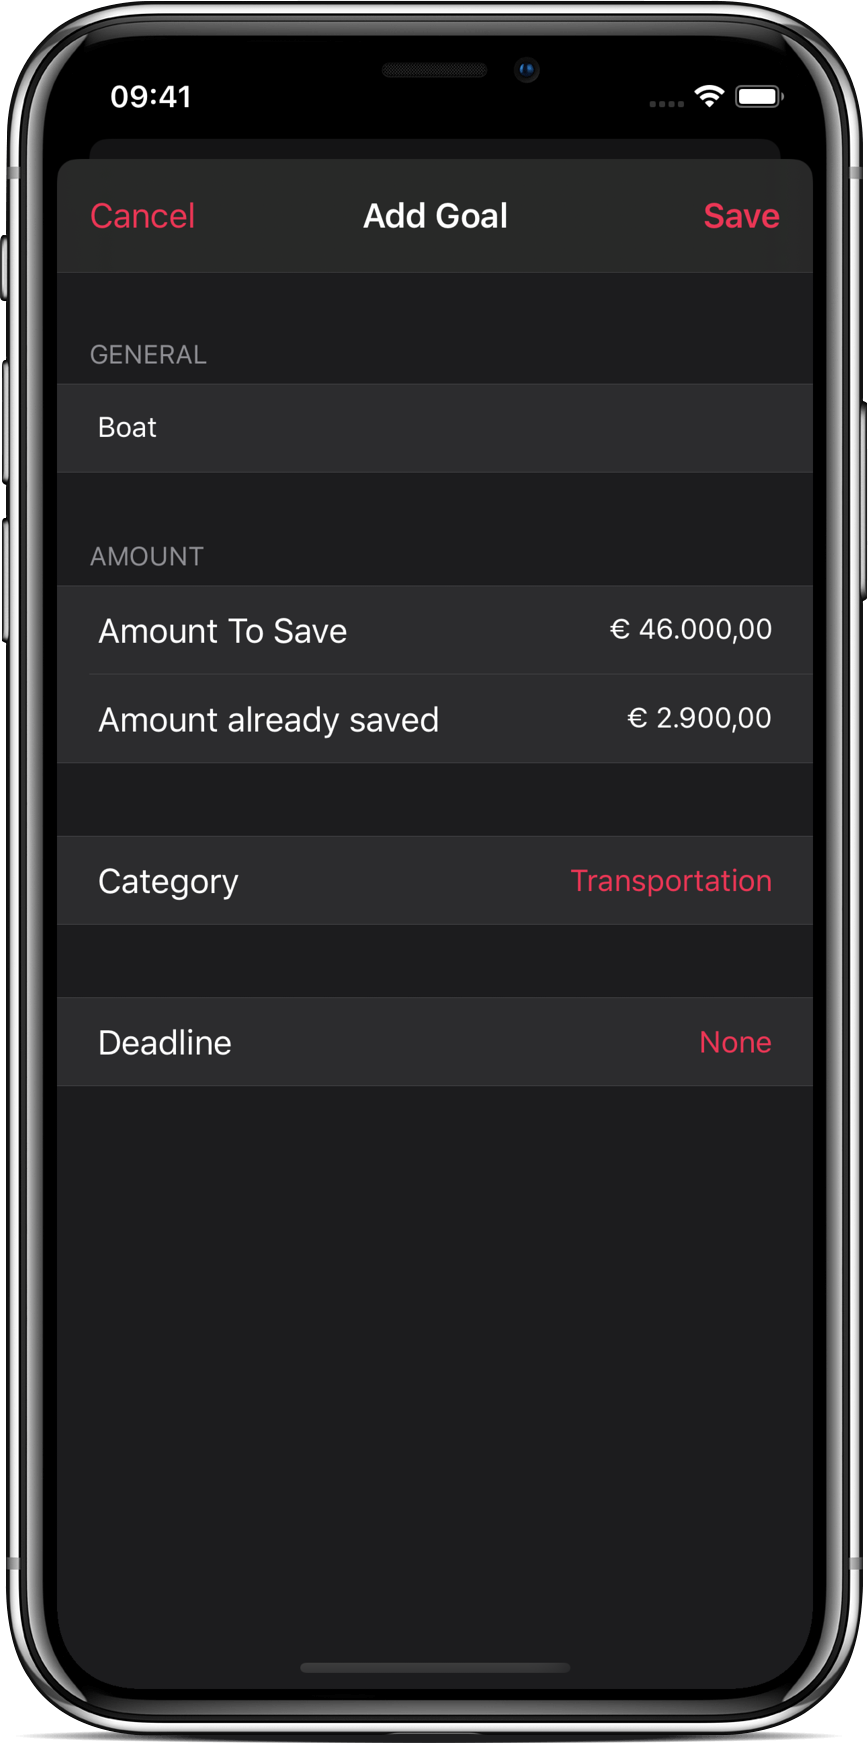
\includegraphics[width=.27\linewidth]{piggy-add-goal}
        \label{fig:piggy:basisfunctionaliteiten:spaardoel-toevoegen}
    }
    \qquad
    \subfloat[Opsomming van alle spaardoelen]{
        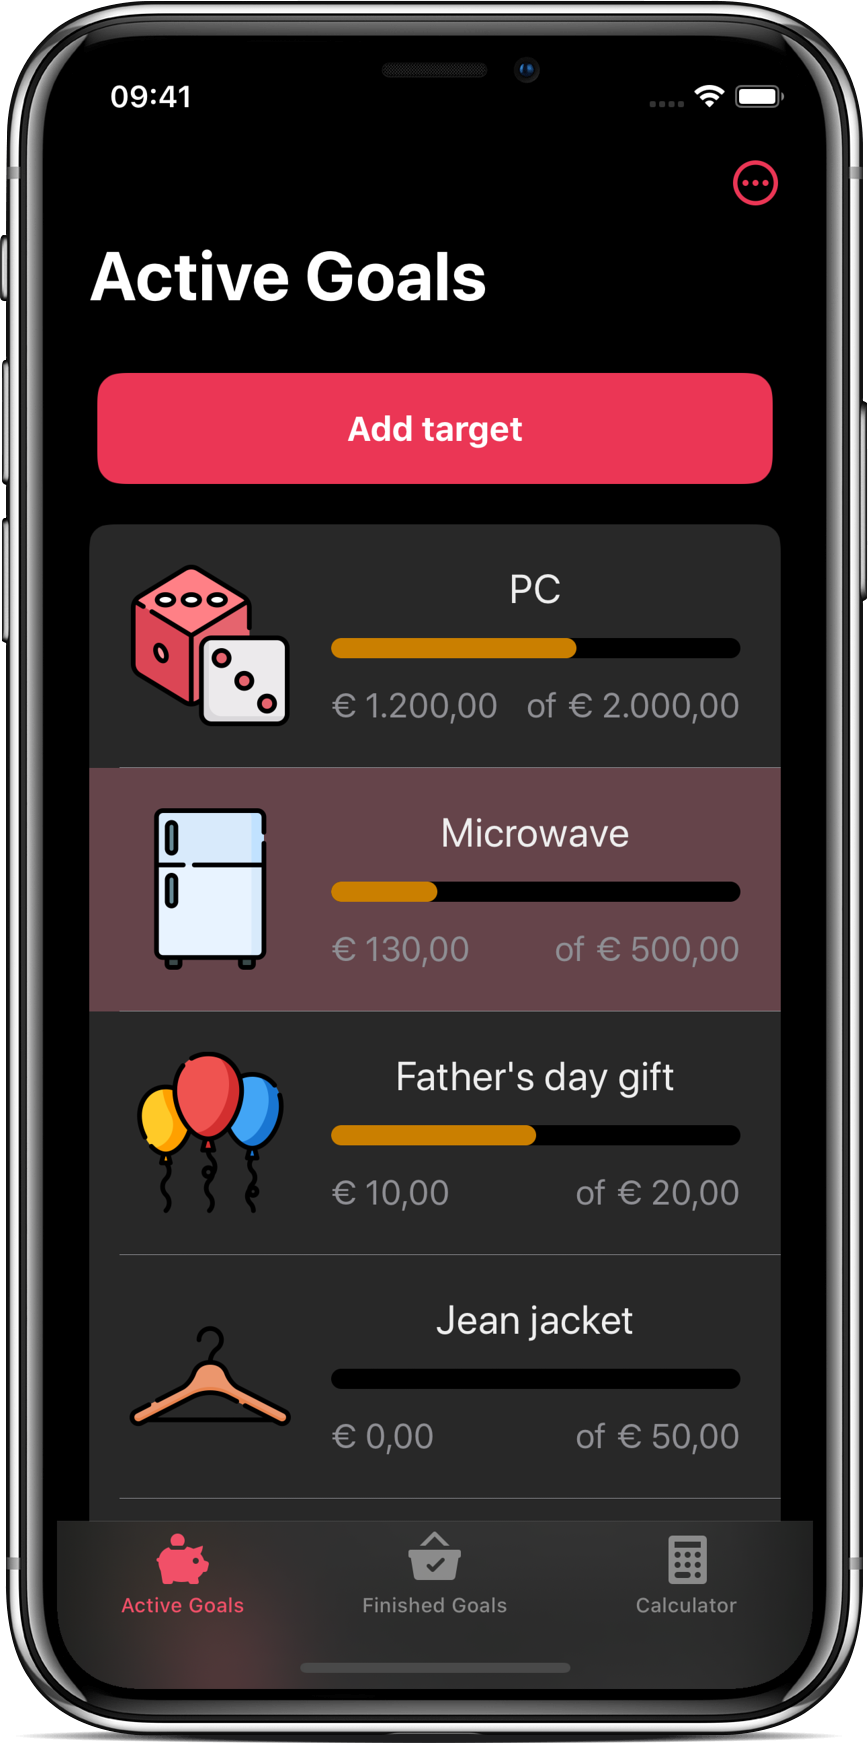
\includegraphics[width=.27\linewidth]{piggy-goals-list}
        \label{fig:piggy:basisfunctionaliteiten:spaardoel-lijst}
    }
    \qquad
    \subfloat[Calculator]{
        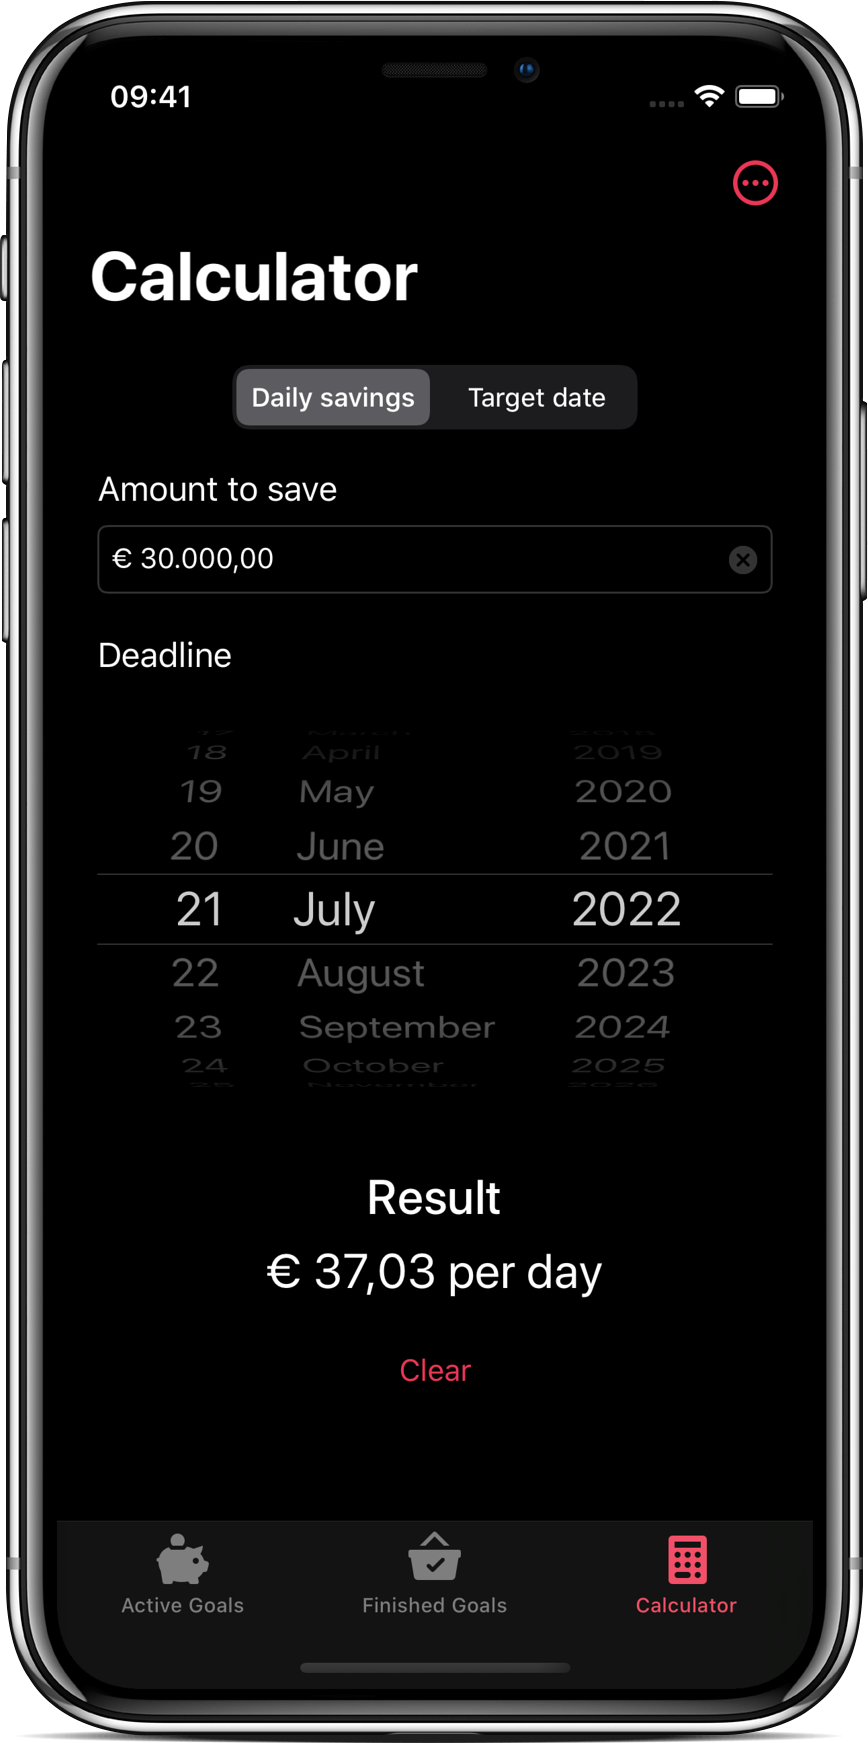
\includegraphics[width=.27\linewidth]{piggy-calculator}
        \label{fig:piggy:basisfunctionaliteiten:calculator}
    }
    \caption{Basisfunctionaliteiten van de proof-of-concept applicatie}
    \label{fig:piggy:basisfunctionaliteiten}
\end{figure}

Eenmaal je een spaardoel hebt toegevoegd kan je telkens een bedrag toevoegen dat je al bijeen gespaard hebt. Dit bedrag wordt bij het totaal opgeteld. Het is mogelijk dit snel te doen door middel van een slider die tot 50 gaat of je kan een extra popover openen waarmee je gedetailleerder je bedrag kan specificeren.

Er zijn ook nog enkele snufjes die iets verder in de menu's verborgen zitten, zoals de mogelijkheid om de applicatie te vergrendelen met een pincode (zie figuur~\ref{fig:piggy:opties:ontgrendel}). Bij de instellingen is het verder ook mogelijk de munteenheid te wijzigen die doorheen de applicatie gehanteerd wordt. Indien je terug van nul wil starten kan je daar ook alle gegevens van de applicatie wissen (zie figuur~\ref{fig:piggy:opties:instellingen}).

\begin{figure}[h!]
    \centering
    \subfloat[Instellingen]{
        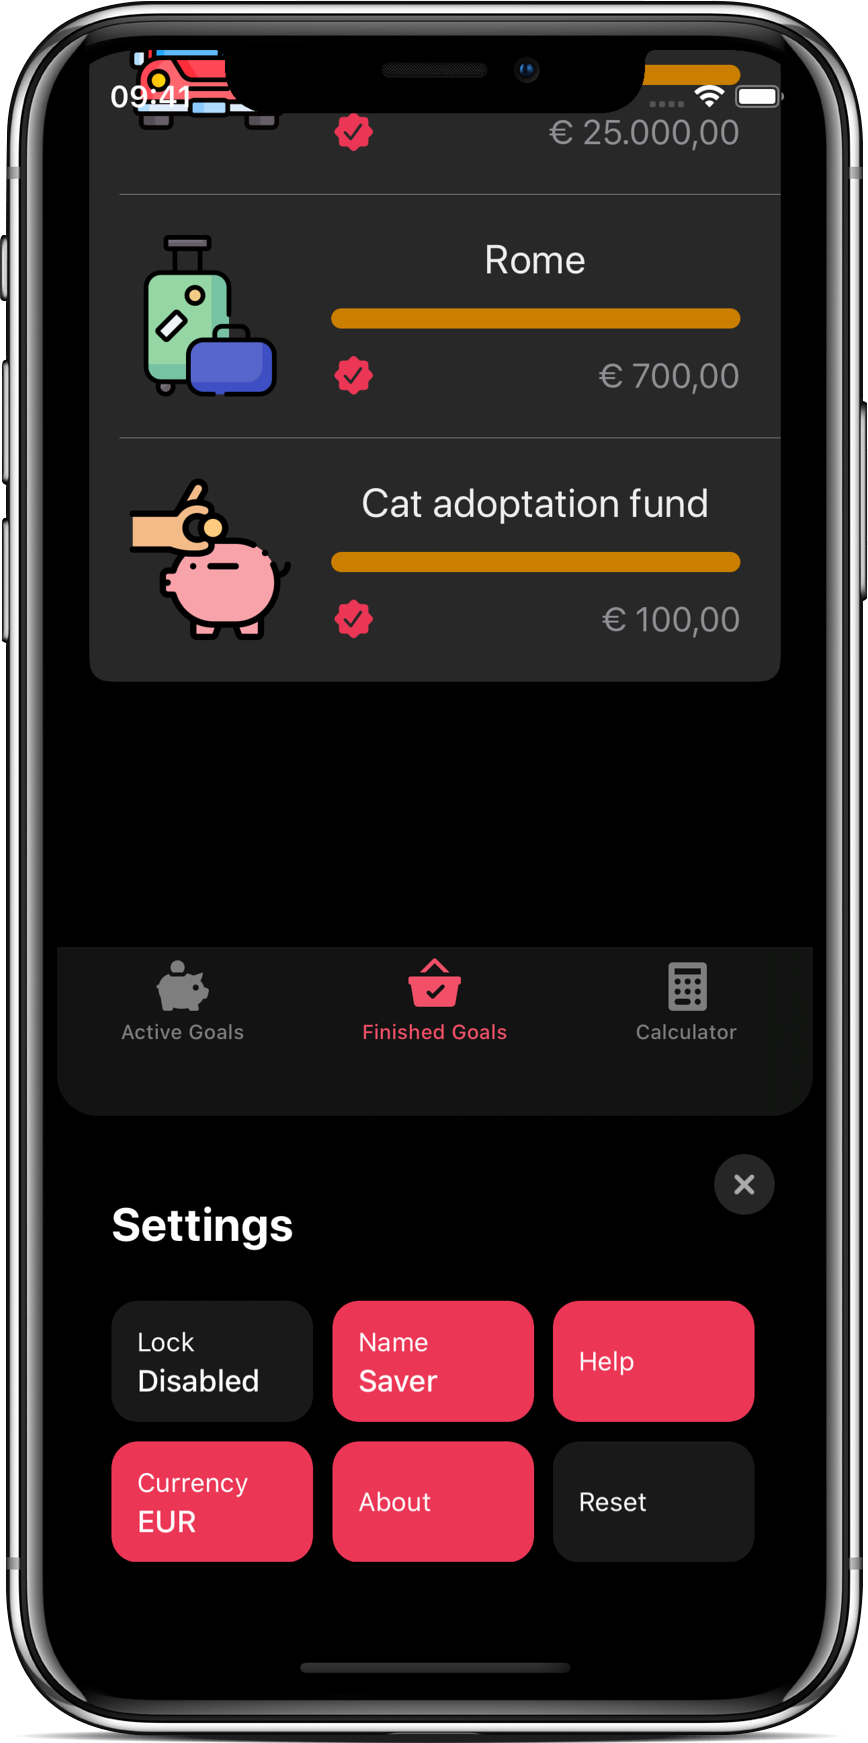
\includegraphics[width=.27\linewidth]{piggy-settings}
        \label{fig:piggy:opties:instellingen}
    }
    \qquad
    \subfloat[Inloggen met Touch ID of Face ID]{
        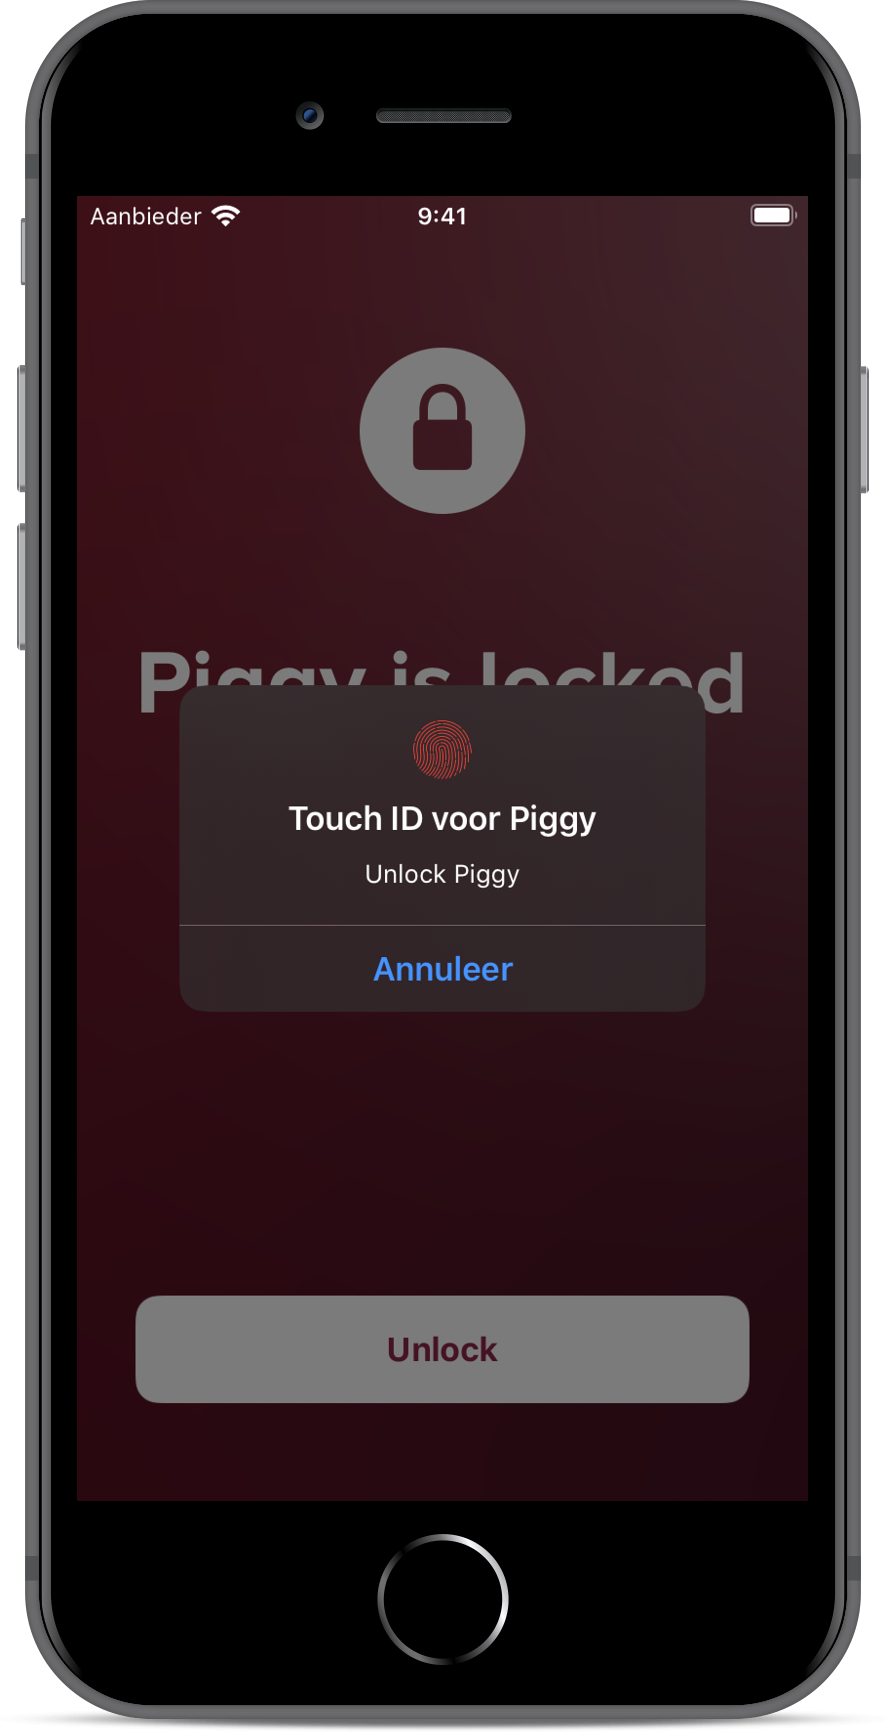
\includegraphics[width=.27\linewidth]{piggy-touchid}
        \label{fig:piggy:opties:ontgrendel}
    }
    \caption{Uitgebreide opties van de proof-of-concept applicatie}
    \label{fig:piggy:opties}
\end{figure}

De applicatie heeft de naam Piggy gekregen, een verwijzing naar piggy bank, de Engelse vertaling voor spaarvarken. Hierbij is ook een bijhorend logo ontworpen (zie figuur~\ref{fig:piggy:icoon}). Doorheen de applicatie maakt men verder gebruik van een roze tint die verwijst naar de kleur van het varkentje verwerkt in het logo. Er werd gekozen voor een alternatieve, gele tint voor elementen die moeten opvallen.

\begin{figure}[h!]
    \centering
    
\includegraphics[width=.2\columnwidth]{piggy-icon}
    \caption{Icoon van Piggy, de proof-of-concept applicatie}
    \label{fig:piggy:icoon}
\end{figure}

\subsection{De learnability elementen}
\label{sec:applicatie:learnability-elementen}

Zoals vooraf aangehaald in hoofdstuk~\ref{sec:experiment} zullen er twee varianten van de proof-of-concept applicatie gemaakt worden. De ene variant bevat alle functionaliteiten maar hierbij is geen uitleg voorzien in de vorm van onboarding en/of in-app training.

De andere applicatie is functioneel niet verschillend aan de applicatie zonder learnability elementen. In deze applicatie worden echter wel enkele aanpassingen gedaan om de learnability van de applicatie te verbeteren in de hoop een positieve invloed te hebben op het klantbehoud. Bij het openen van deze applicatie wordt de gebruiker gegroet met een welkomstbericht en start er direct een rondleiding aan de hand van tooltips die voorzien zijn van uitleg (zie hoofdstukken~\ref{sec:onboarding:welkomstberichten},~\ref{sec:onboarding:rondleidingen} en figuur~\ref{fig:piggy:onboarding}). Wanneer de gebruiker in de applicatie meer uitleg wenst kan hij/zij de rondleiding van bepaalde onderdelen herstarten door het vraagteken-icoon aan te klikken in de navigatiebalk. Als laatste redmiddel is er ook een uitgebreide help-sectie voorzien (zie hoofdstuk~\ref{sec:in-app-training} en figuur~\ref{fig:piggy:help}).

\begin{figure}[h!]
    \centering
    \subfloat[Hulp bij het starten met het gebruik wanneer de applicatie voor de eerste maal start]{
        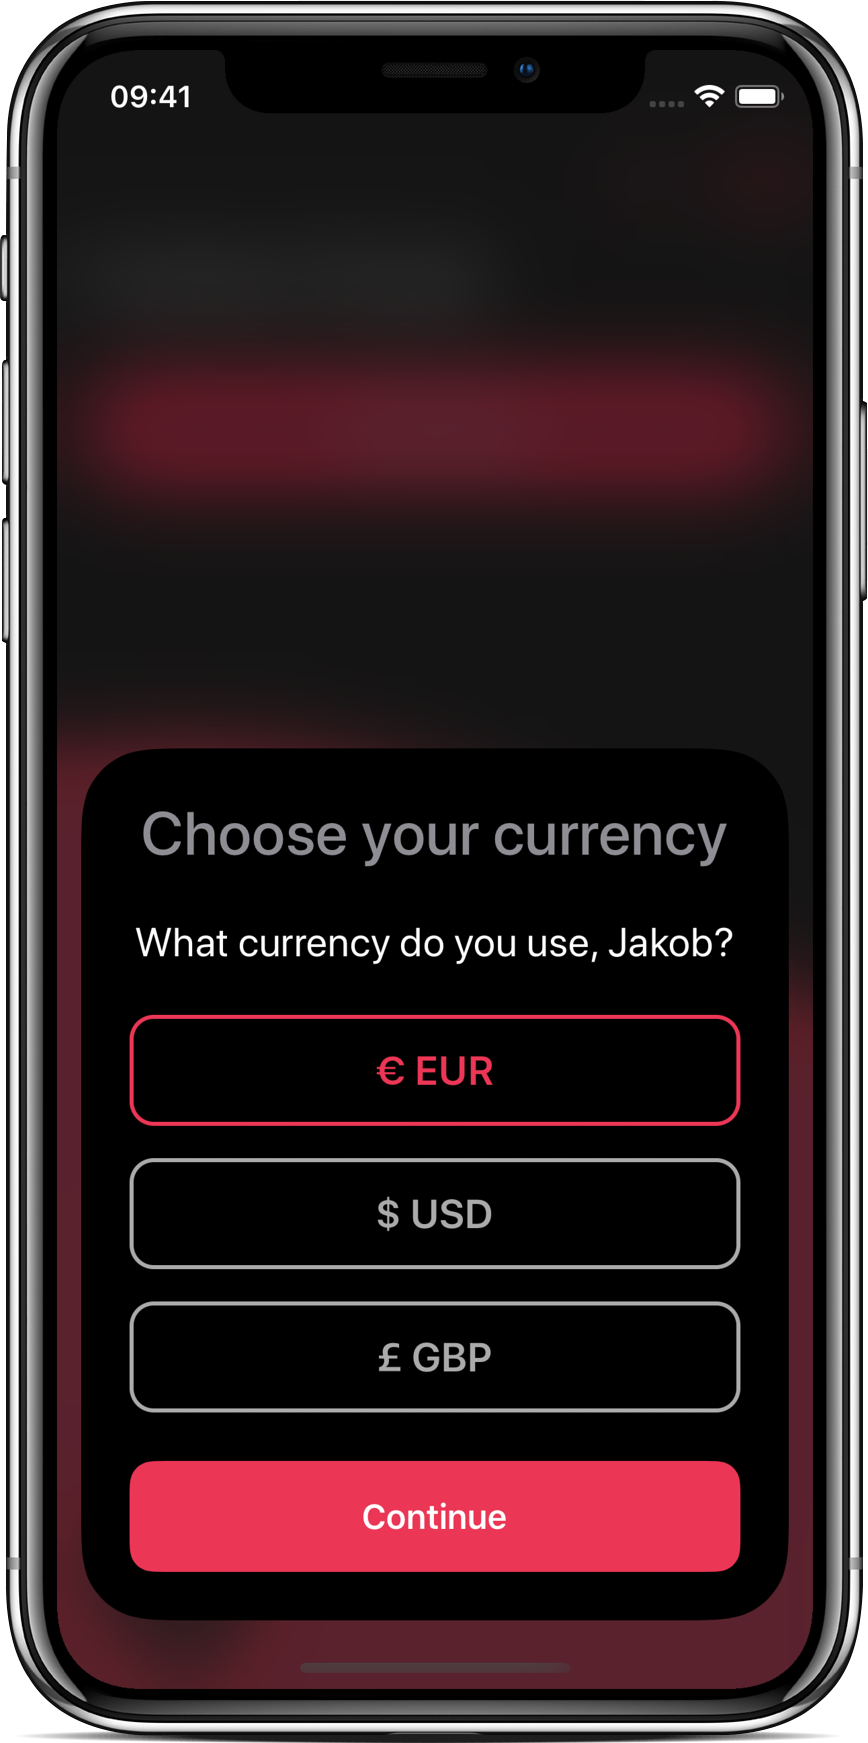
\includegraphics[width=.27\linewidth]{piggy-onboarding}
        \label{fig:piggy:onboarding:welkom}
    }
    \qquad
    \subfloat[De rondleiding toont alle belangrijke functionaliteiten]{
        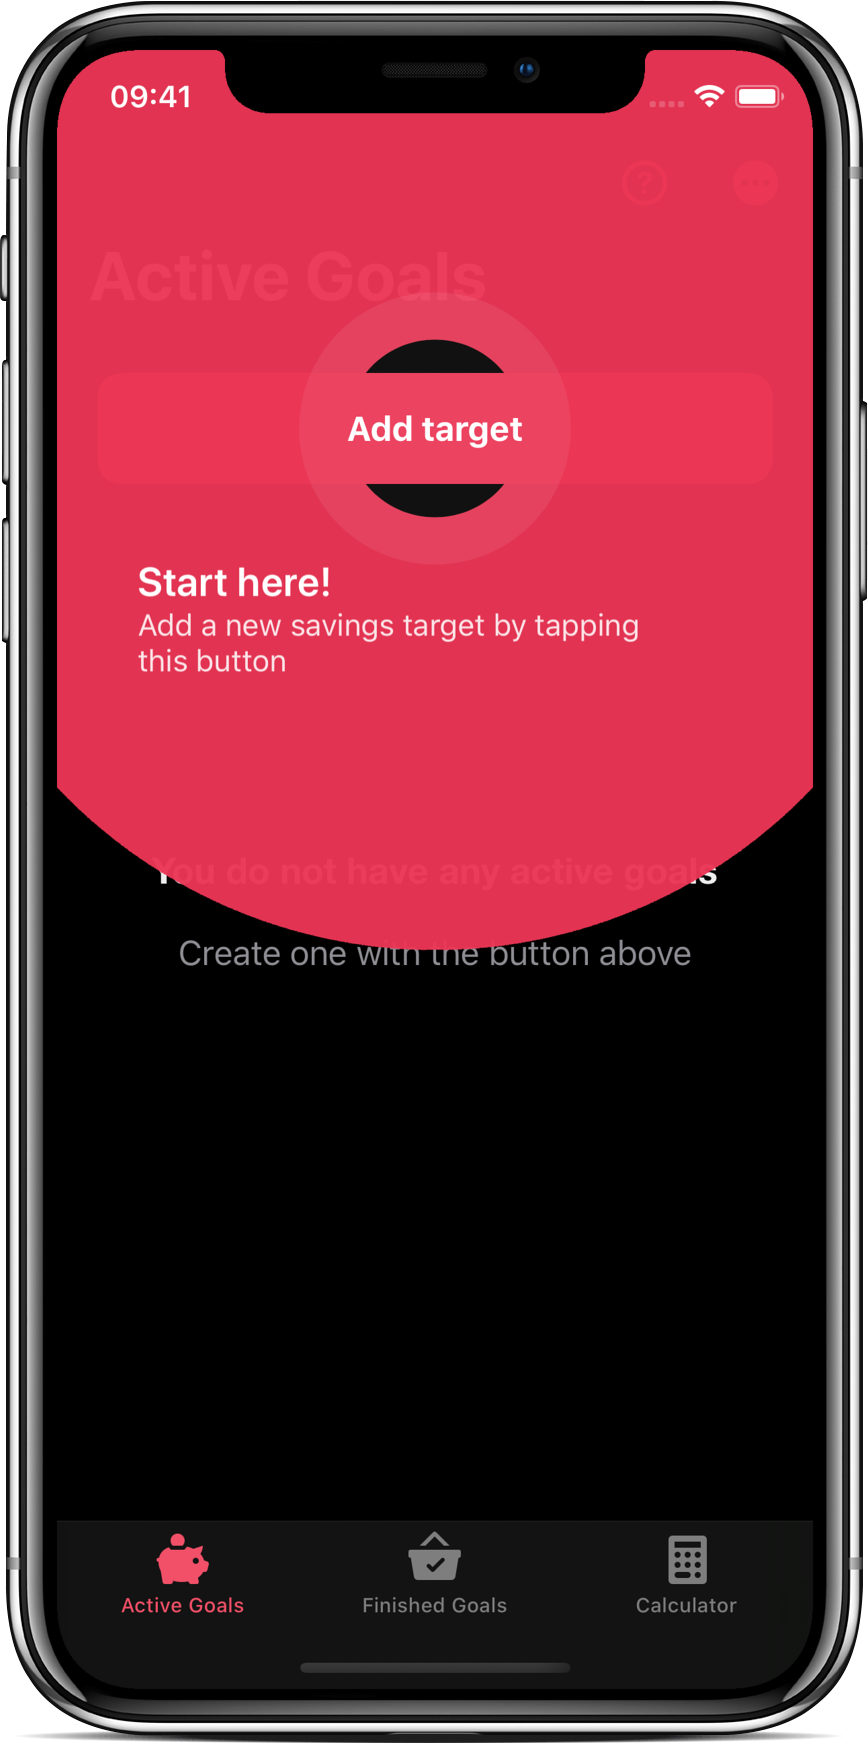
\includegraphics[width=.27\linewidth]{piggy-showcase}
        \label{fig:piggy:onboarding:functies}
    }
    \caption{Een rondleiding doorheen de proof-of-concept applicatie}
    \label{fig:piggy:onboarding}
\end{figure}

\begin{figure}[h!]
    \centering
    \subfloat[Een lijst met alle onderwerpen]{
        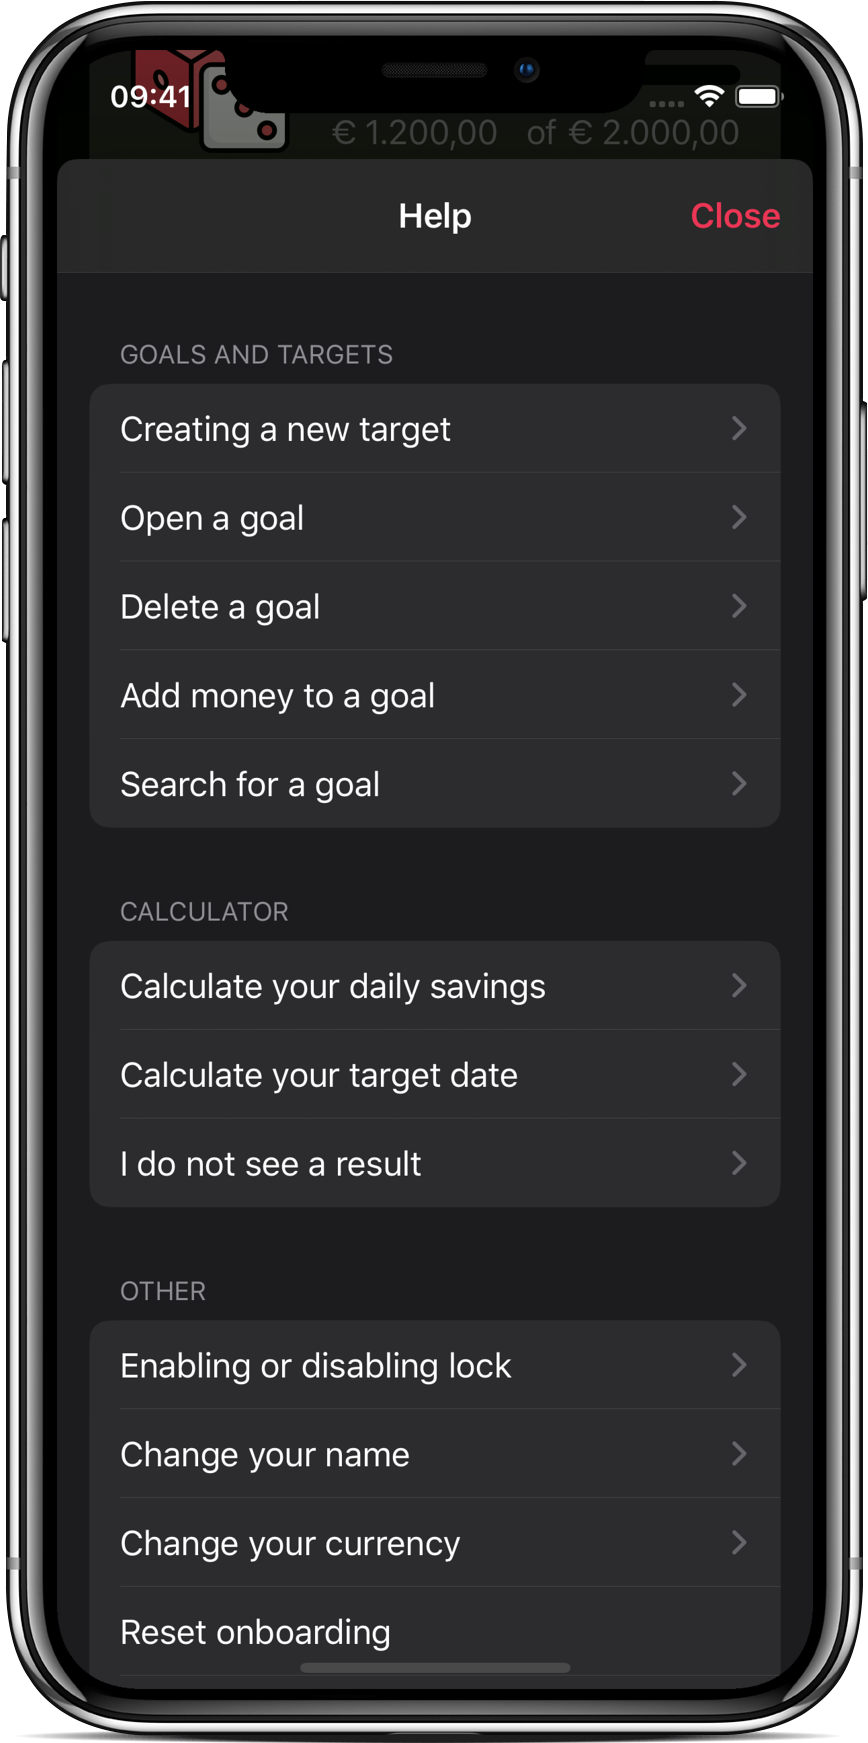
\includegraphics[width=.27\linewidth]{piggy-help}
        \label{fig:piggy:help:lijst}
    }
    \qquad
    \subfloat[Een bepaalde functie grondig uitgelegd]{
        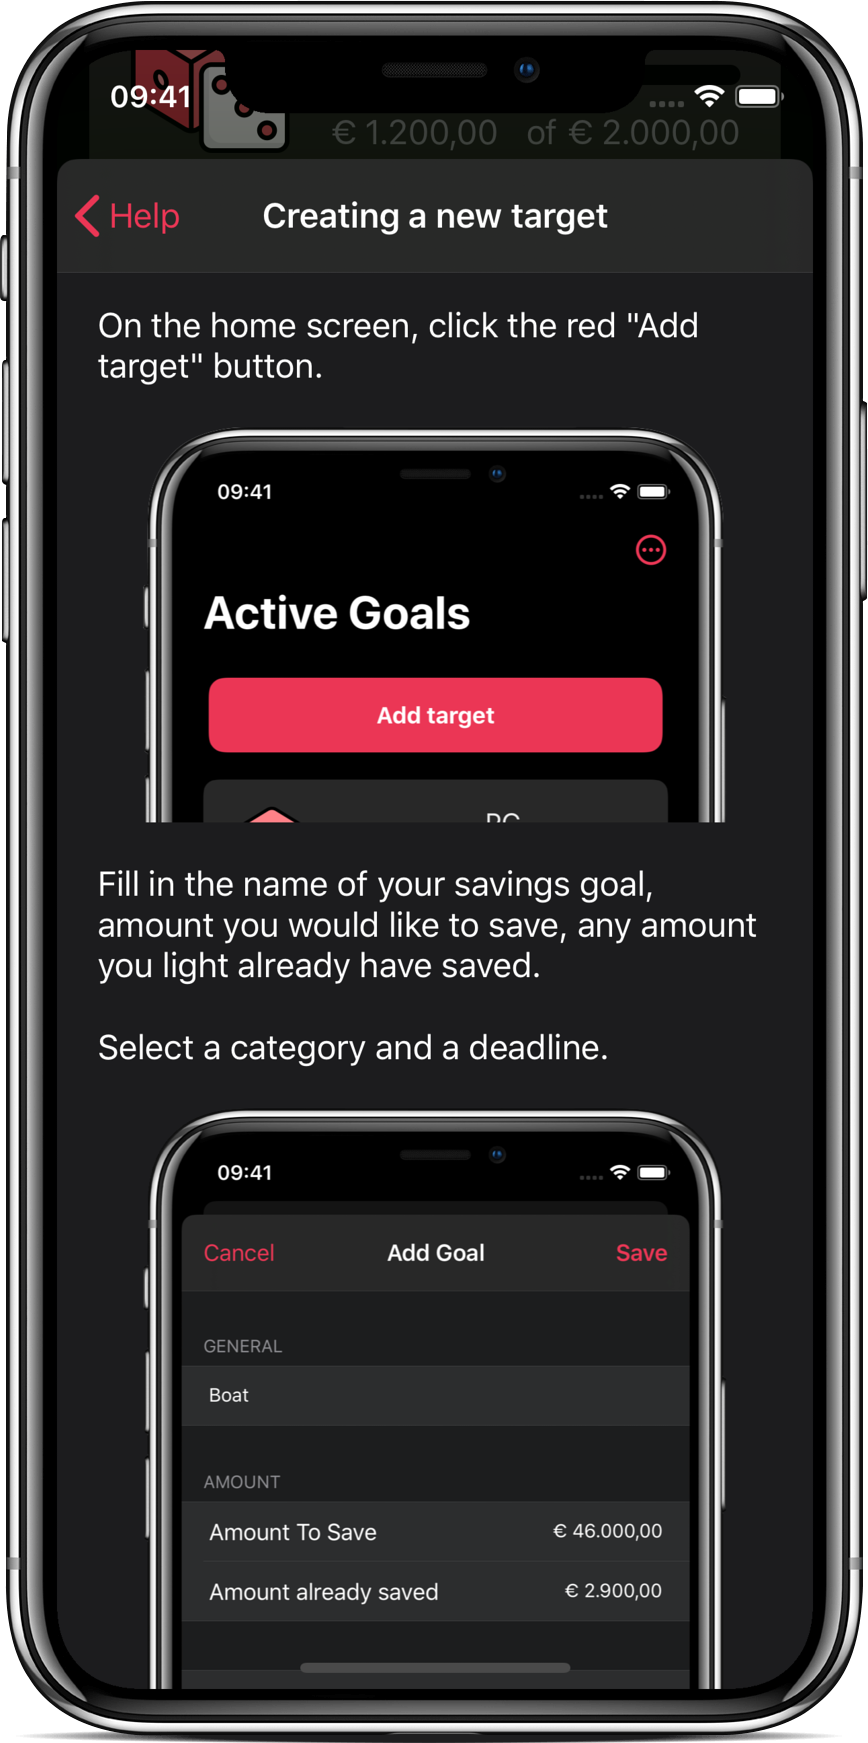
\includegraphics[width=.27\linewidth]{piggy-help-article}
        \label{fig:piggy:help:artikel}
    }
    \caption{Uitgebreide help-sectie in de proof-of-concept applicatie}
    \label{fig:piggy:help}
\end{figure}

Deze onboarding en hulp doorheen de applicatie beperkt zich tot de essentiële onderdelen ervan. De gebruiker kan vlot starten met het gebruik van de applicatie. Gaandeweg komen er nog enkele tooltips tevoorschijn om zo de aandacht te vestigen op een onderdeel dat de gebruiker net ontdekt heeft (bijvoorbeeld: de gebruiker wil een nieuw spaardoel creëren en de bijhorende interface komt tevoorschijn) (zie hoofdstuk~\ref{sec:onboarding:types:progressief}). Er werd bij het uitdenken van de onboarding aandacht gehecht aan de vijf basisprincipes uit hoofdstuk~\ref{sec:onboarding:start}.

Deze onboarding is een voorbeeld van een functiegerichte onboarding. De focus ligt voornamelijk bij het uitleggen van functionaliteiten aan de gebruiker zodat deze vlot met de applicatie overweg kan (zie hoofdstuk~\ref{sec:onboarding:types:functie}).

Vooraleer er werd gestart aan de usability tests werd deze applicatie grondig getest op onduidelijkheden doorheen de onboarding.

\subsection{Ontwikkeling}
\label{sec:applicatie:ontwikkeling}

Er werd gekozen om de applicatie te schrijven voor het mobiele platform van Apple (iOS) omdat veel gebruikers met grote diversiteit hiermee bekend zijn. De applicatie werd geschreven in de programmeertaal Swift 5 en draait op iOS 13 of hoger.

\textit{De volledige broncode van de applicatie is te raadplegen op \url{https://github.com/JakobLierman/piggy}.}

\section{De test afnemen}
\label{sec:test-afnemen}

Vooraleer de test wordt afgenomen, vulden de participanten al enkele vragen in. Enerzijds gingen deze vragen over of ze al dan niet in aanmerking kwamen om deel te nemen aan dit onderzoek, anderzijds gingen deze vragen over hun demografische gegevens (zie bijlage~\ref{bijlage:deelnameformulier}).

De standaardprocedure voor het afnemen van deze test gaat als volgt: de participanten worden via een videogesprek de procedure uitgelegd. Afhankelijk van de groep waarvan de participant deel uitmaakt, krijgt deze de applicatie met of zonder de learnability elementen. De participanten voeren achtereenvolgens een aantal opdrachten uit om de usability van de applicatie in kaart te brengen. Tijdens deze opdrachten observeert de moderator het gedrag van de participanten. Na afloop vullen ze de~\acrshort{acr:sus} vragenlijst in (zie bijlage~\ref{bijlage:sus}).

Tenslotte wordt de opzet van het onderzoek uitgelegd. Hierna krijgt de participant nog even tijd om de andere applicatie uit te testen (afhankelijk van in welke groep de participant zich bevindt). Op basis van deze twee ervaringen mag de participant aangeven welke van de twee applicatie hij of zij prefereert.
